\section{Fundamentals of plotting in Origin}
	An installation of Origin comes with a collection of sample data which is recommended for a beginner to learn the fundamentals of plotting and subsequent customization. In order to access this collection of sample data, one can go to the main menu and click \verb|Help| \verb|>| \verb|Open Folder| \verb|>| \verb|Sample Folder|.
	
	This would open up the \verb|Sample| folder in a Windows Explorer.
	\begin{figure}[h!]
		\centering
		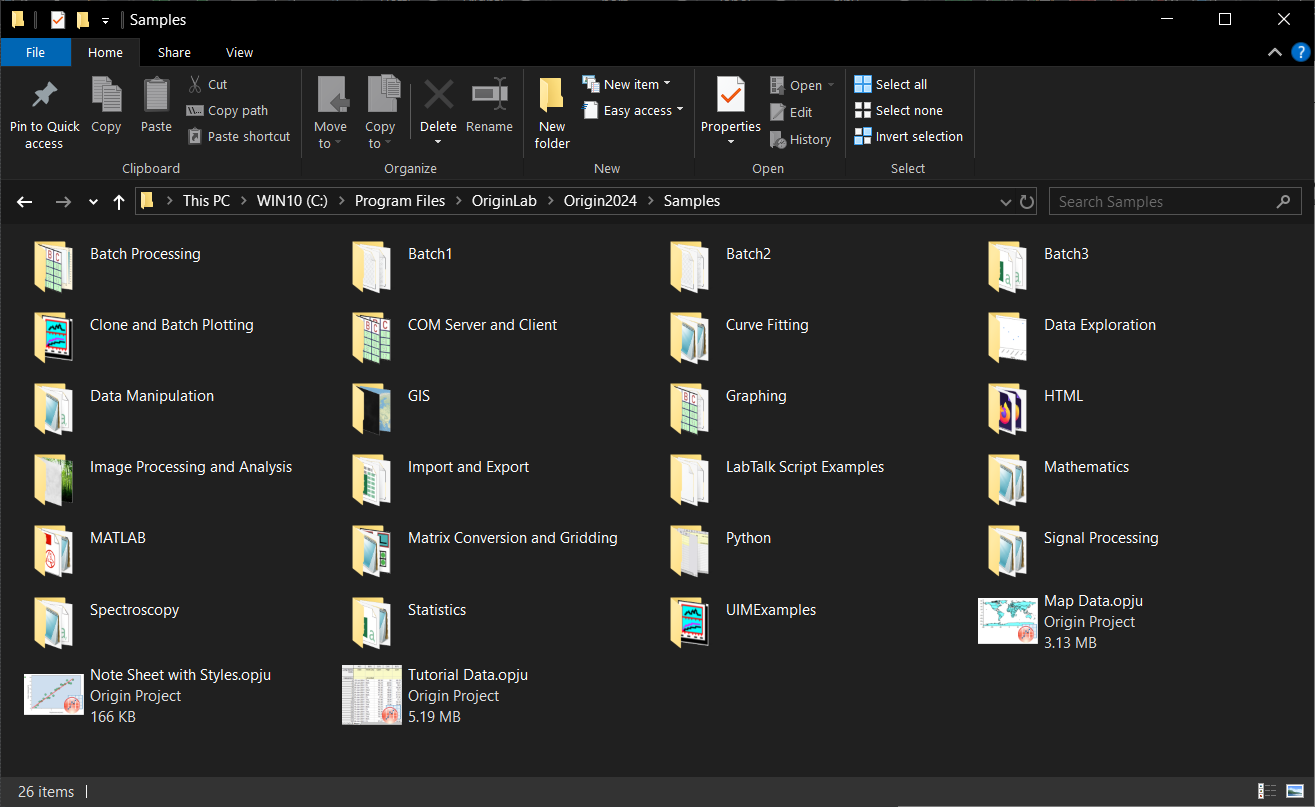
\includegraphics[width=0.8\textwidth]{figures/fig_samples-folder.png}
	\end{figure}
	
	\subsection{Plotting the first graph} \label{ssec:first-graph}
		
		\subsubsection{Importing data from sample folder}
			\begin{enumerate}[I.]
				\item Launch Origin to find the default empty workbook which contains a single worksheet with two columns.
				\begin{figure}[h!]
					\centering
					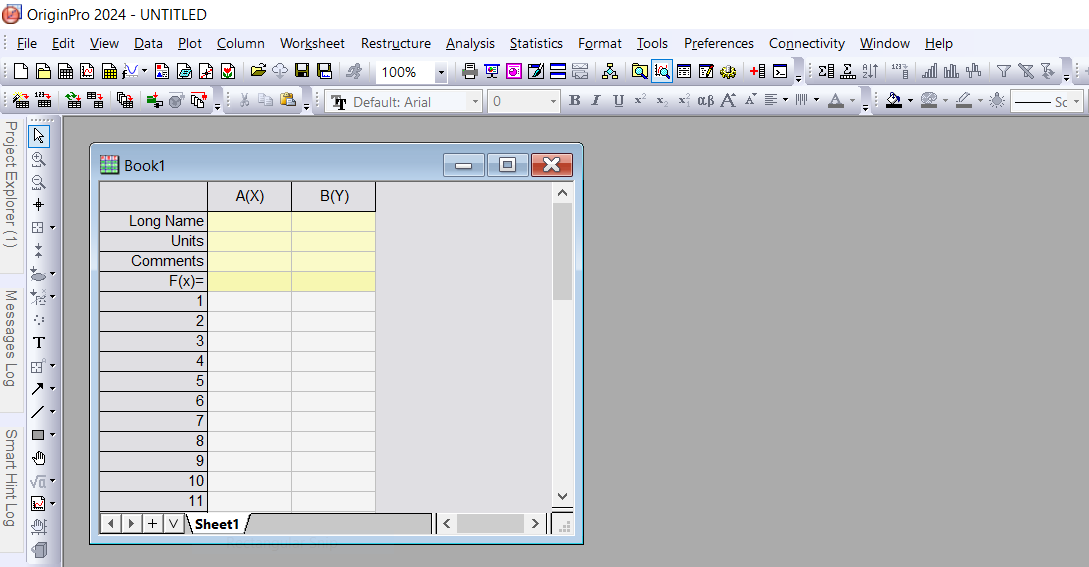
\includegraphics[width=0.8\textwidth]{figures/fig_default-project.png}
				\end{figure}
				
				\item Navigate into the \verb|Curve Fitting| folder in the \verb|Sample| folder.
				\begin{figure}[h!]
					\centering
					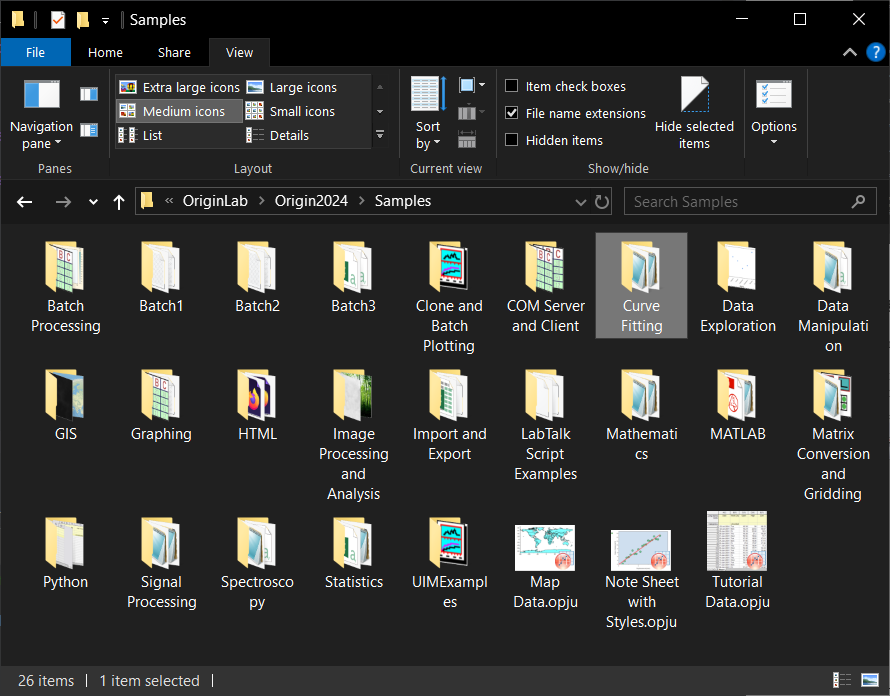
\includegraphics[width=0.5\textwidth]{figures/fig_sample-curvfit-folder.png}
				\end{figure}
				
				\item Locate any of the DAT files, such as \verb|Sensor01.dat|. Then drag and drop it into the Origin workbook.
				\begin{figure}[h!]
					\centering
					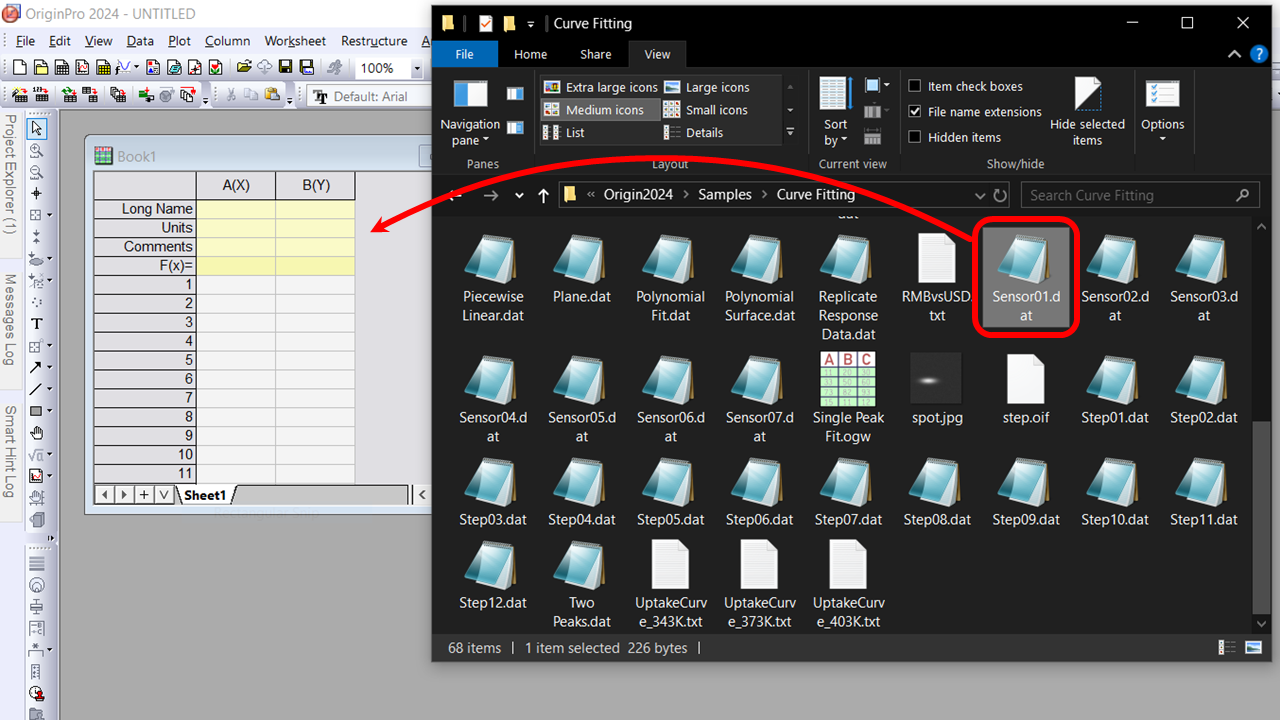
\includegraphics[width=0.8\textwidth]{figures/fig_import-drag.png}
				\end{figure}
				
				\item This would import the data from the DAT file into the workbook.
				\begin{figure}[h!]
					\centering
					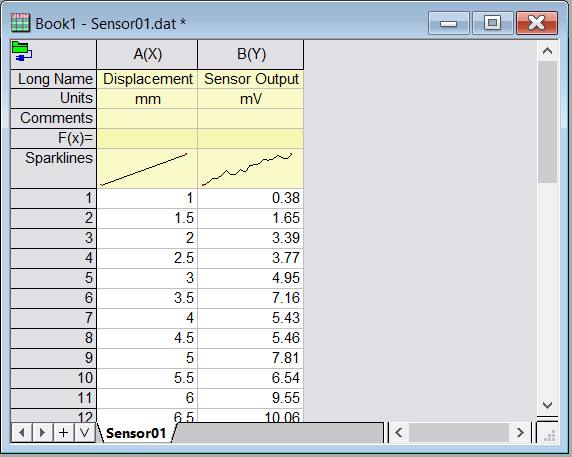
\includegraphics[width=0.4\textwidth]{figures/fig_drag-import.png}
				\end{figure}
			\end{enumerate}
			
		\subsubsection{Plotting the graph}
			\begin{enumerate}[I.]
				\item Click on the header of column B to select the entire column.
				\begin{figure}[h!]
					\centering
					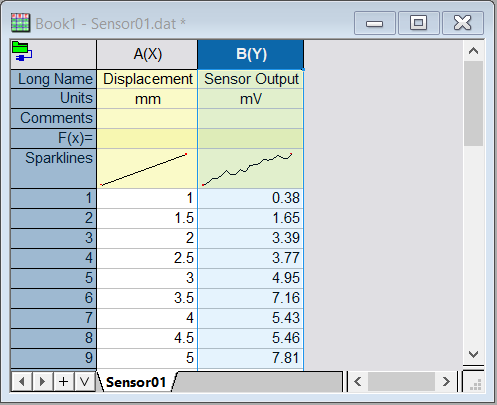
\includegraphics[width=0.4\textwidth]{figures/fig_basic-plot-01.png}
				\end{figure}
				
				\item From the main menu, we click \verb|Plot > Basic 2D > Line|.
				\begin{figure}[h!]
					\centering
					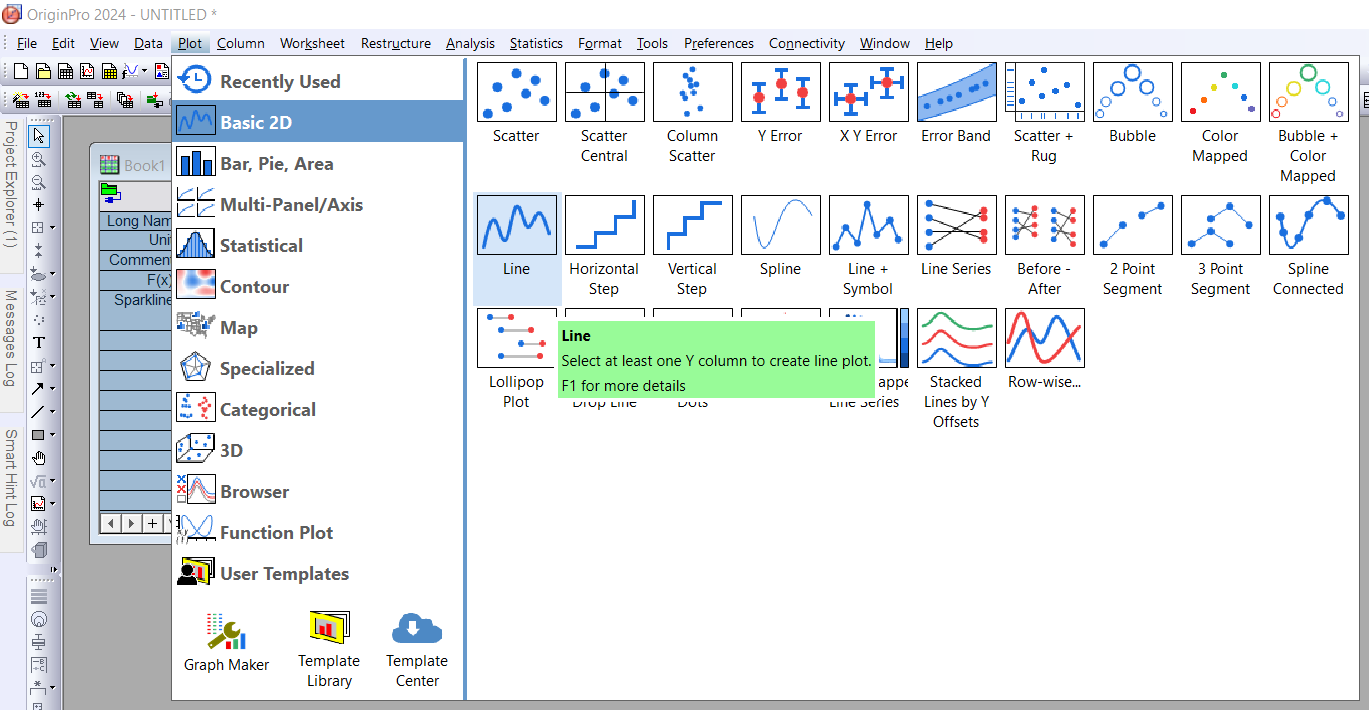
\includegraphics[width=0.8\textwidth]{figures/fig_basic-plot-02.png}
				\end{figure}
				
				\item This produces a basic 2D plot.
				\begin{figure}[h!]
					\centering
					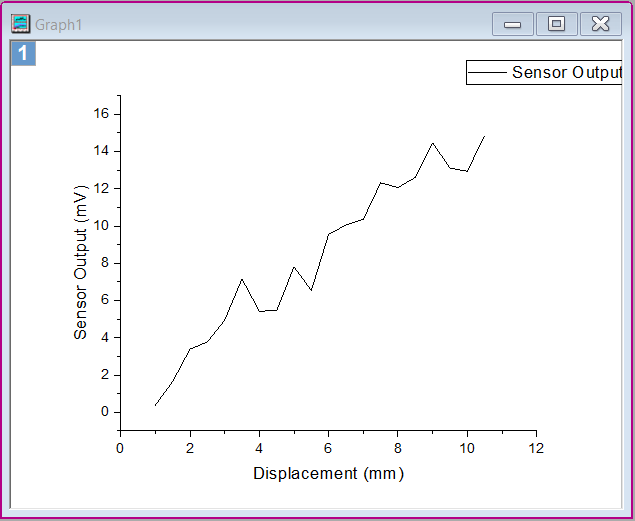
\includegraphics[width=0.5\textwidth]{figures/fig_basic-plot-03.png}
				\end{figure}
			\end{enumerate}
			
		\subsubsection{Basic customization of the plot}
			\begin{enumerate}[I.]
				\item Click on the $x$-axis so that the mini toolbar pops up. Then click \verb|Show Gridlines > Both|.
				\begin{figure}[h!]
					\centering
					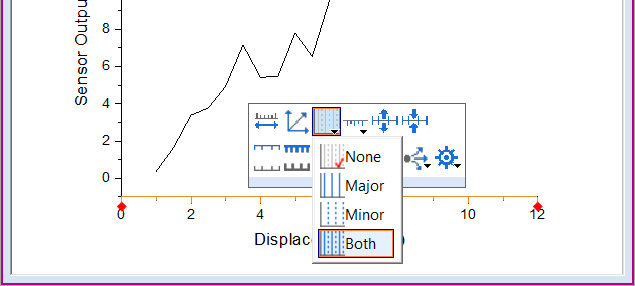
\includegraphics[width=0.6\textwidth,frame]{figures/fig_plot-basic-custom-01.png}
				\end{figure}
				
				\item Repeat the above step on the $y$-axis to get a plot with major and minor gridlines.
				\begin{figure}[h!]
					\centering
					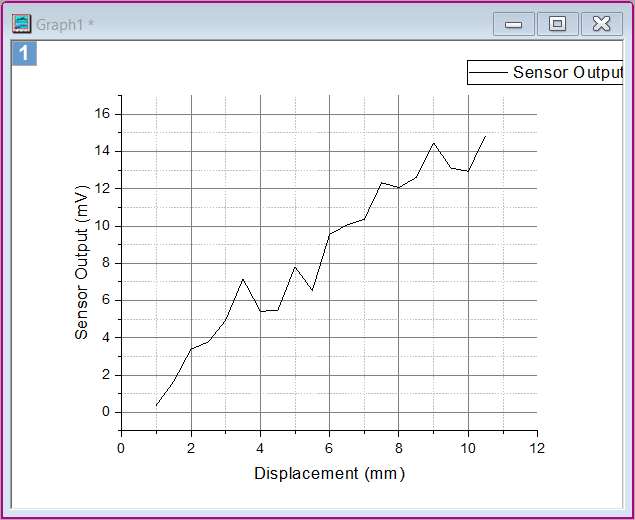
\includegraphics[width=0.5\textwidth]{figures/fig_plot-basic-custom-02.png}
				\end{figure}
				
				\item Click on the line plot so that the mini toolbar pops up. Then click on the \verb|Line Color| button to select a colour, say blue. Also set the \verb|Line Thickness| to a larger value, say 4.
				\begin{figure}[h!]
					\centering
					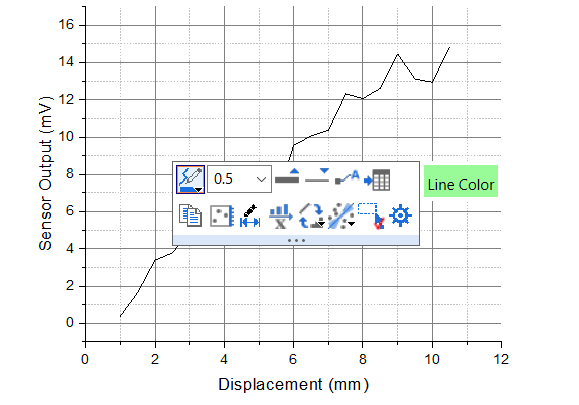
\includegraphics[width=0.45\textwidth,frame]{figures/fig_plot-basic-custom-03.png}
					\hfill
					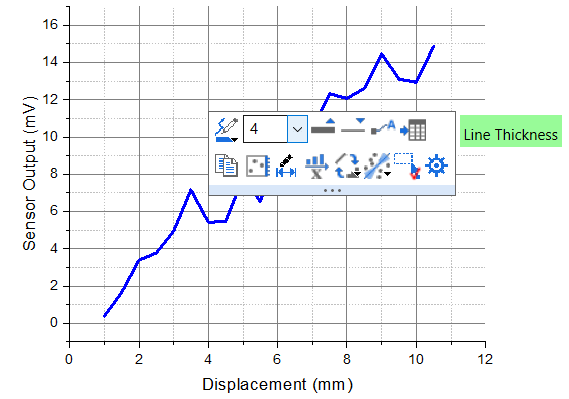
\includegraphics[width=0.45\textwidth,frame]{figures/fig_plot-basic-custom-04.png}
				\end{figure}
				
				\newpage
				\item Click on the plot background (ensure that the plot or the gridlines are not clicked), click on \verb|Layer Background Color| and then select some background colour, such as light yellow.\vspace{-3ex}
				\begin{figure}[h!]
					\centering
					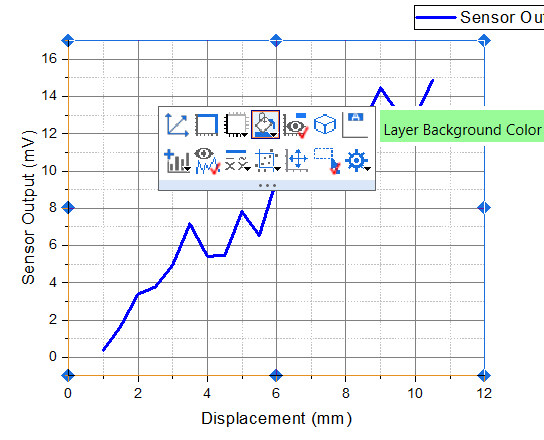
\includegraphics[width=0.45\textwidth,frame]{figures/fig_plot-basic-custom-05.png}
					\hfill
					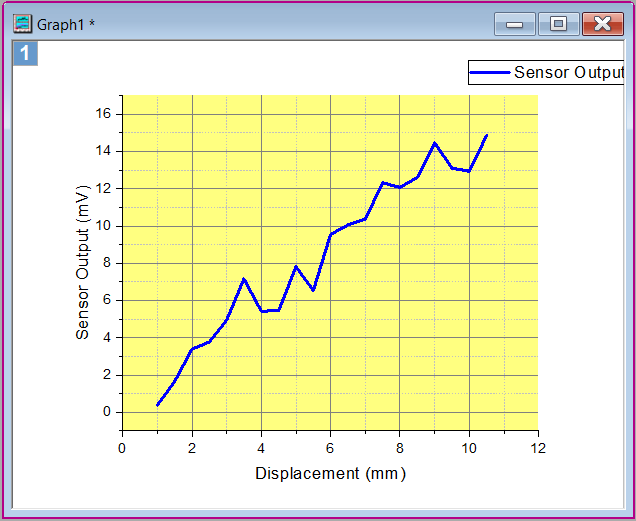
\includegraphics[width=0.45\textwidth]{figures/fig_plot-basic-custom-06.png}
				\end{figure}
				
				\item We can create a bounding box by displaying opposite axes and removing the tick marks. To do so, we click on any of the tick labels on the $x$-axis and then click \verb|Show Opposite Axis| on the pop-up menu. On the pop-up menu of the opposite axis, we click on the \verb|Tick Style| button and then on \verb|None|.\vspace{-1.5ex}
				\begin{figure}[h!]
					\centering
					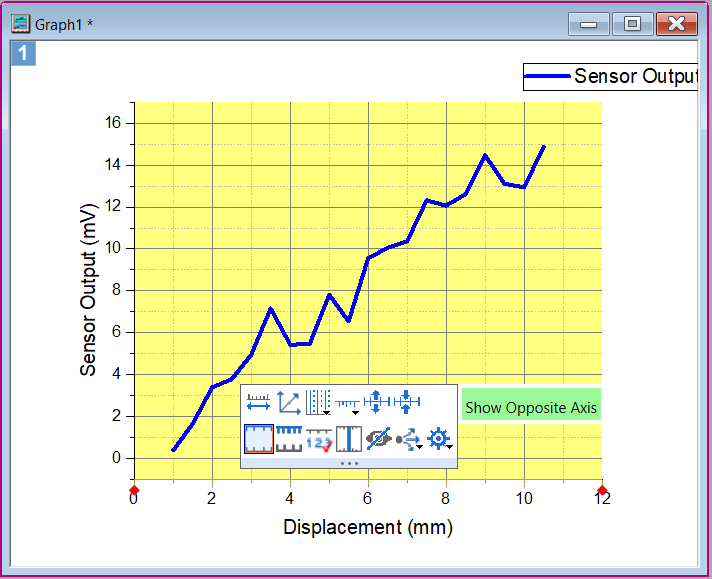
\includegraphics[width=0.45\textwidth]{figures/fig_plot-basic-custom-07.png}
					\hfill
					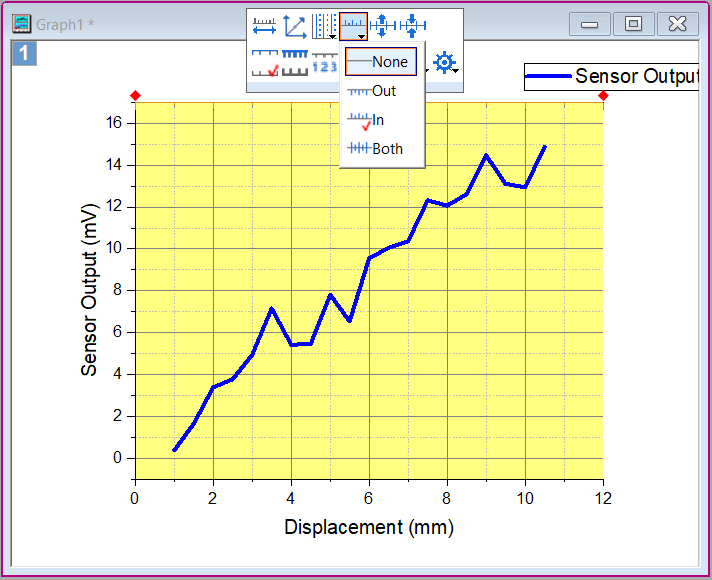
\includegraphics[width=0.45\textwidth]{figures/fig_plot-basic-custom-08.png}
				\end{figure}
				
				\item Repeating the above step for the $y$-axis gives us the desired bounding box around the graph.\vspace{-3ex}
				\begin{figure}[h!]
					\centering
					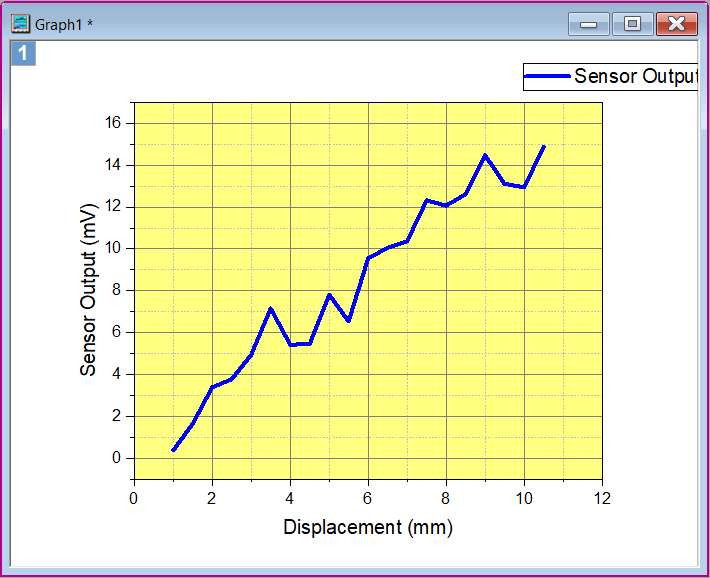
\includegraphics[width=0.5\textwidth]{figures/fig_plot-basic-custom-09.png}
				\end{figure}
				
				\item We can remove the graph legend by clicking on it and pressing the delete button on the keyboard.\vspace{-2ex}
				\begin{figure}[h!]
					\centering
					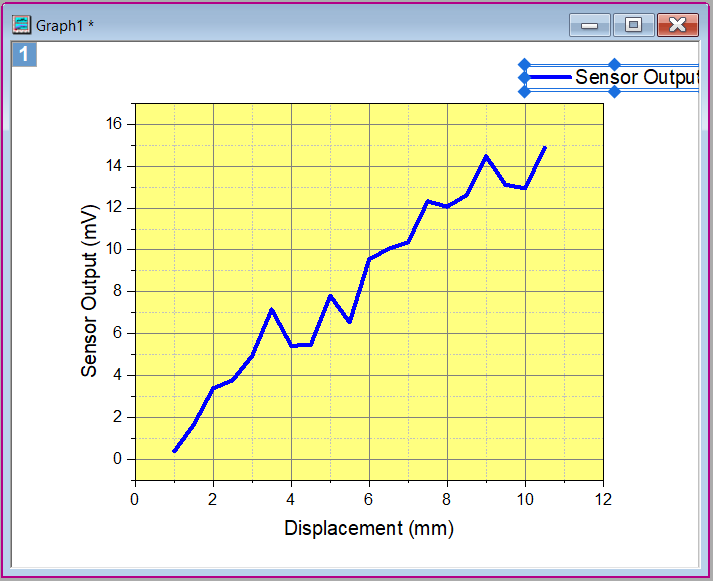
\includegraphics[width=0.45\textwidth]{figures/fig_plot-basic-custom-10.png}
					\hfill
					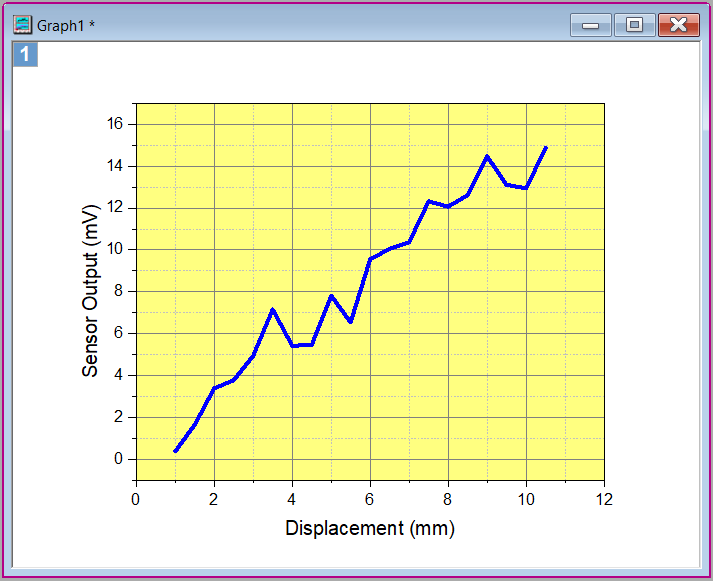
\includegraphics[width=0.45\textwidth]{figures/fig_plot-basic-custom-11.png}
				\end{figure}
				
				\item To modify the typeface of the tick labels, we click on any of the tick labels and on the pop-up menu, we set the font size (here, 22) and the font (here, Cambria). Likewise, we click on the axis label and on the pop-up menu, we set the font size (here, 26) and the font (here, Cambria).\vspace{-2ex}
				\begin{figure}[h!]
					\centering
					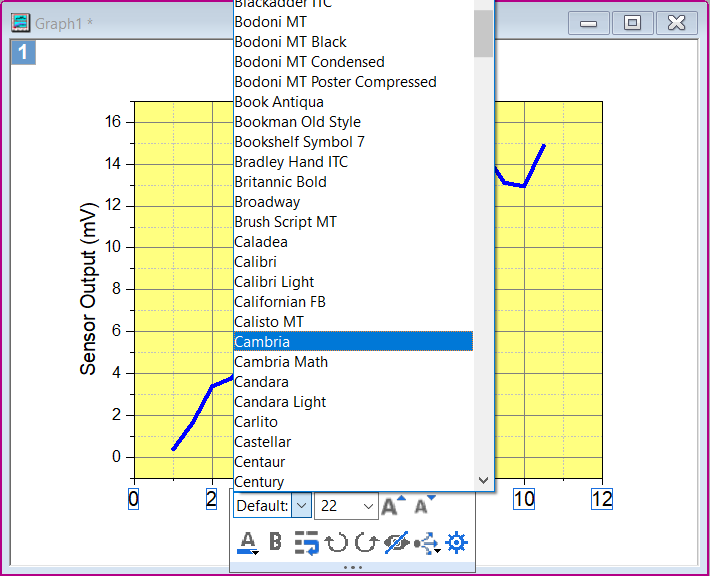
\includegraphics[width=0.45\textwidth]{figures/fig_plot-basic-custom-12.png}
					\hfill
					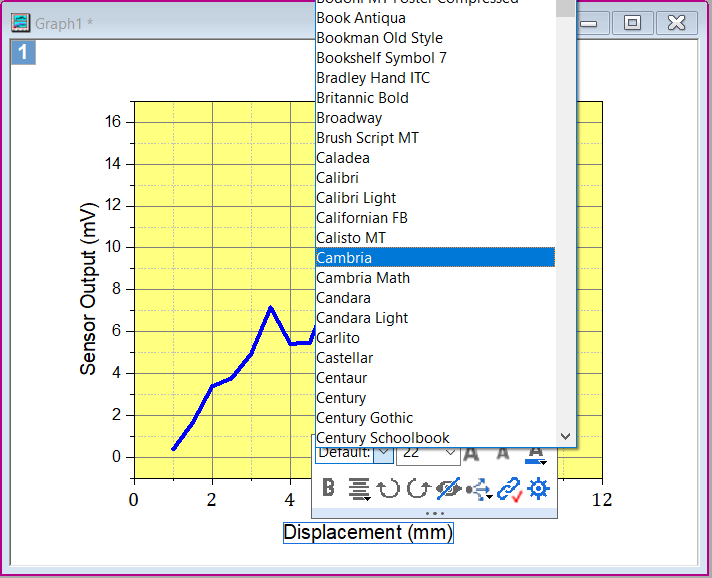
\includegraphics[width=0.45\textwidth]{figures/fig_plot-basic-custom-13.png}
				\end{figure}
				
				\item We repeat the above step for the $y$-axis tick and axis labels to obtain a graph with the desired aesthetics.\vspace{-2ex}
				\begin{figure}[h!]
					\centering
					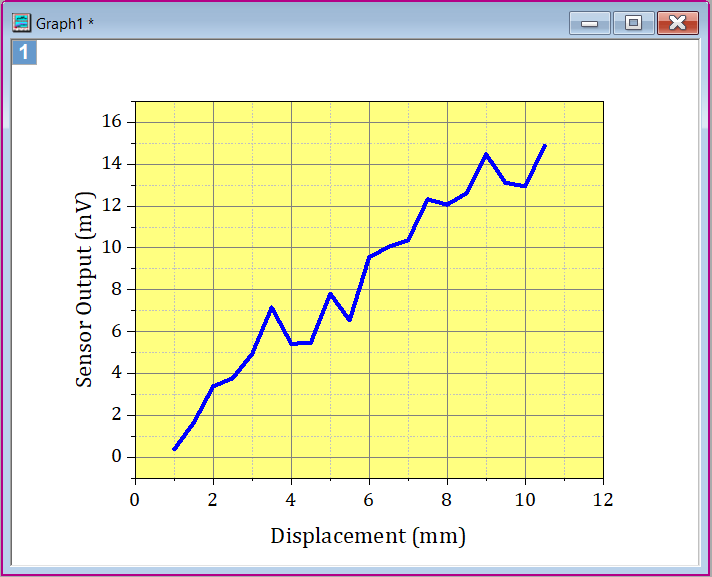
\includegraphics[width=0.5\textwidth]{figures/fig_plot-basic-custom-14.png}
				\end{figure}
				
				\item Finally, export the graph into an image file, we right-click on the graph's title bar, and then click on \verb|Export Graph as Image|. Then in the export graph dialog, we set \verb|Image Type = PNG|, \verb|File Name| as appropriate (here, \verb|my-line-plot|), and \verb|File Path| to be the appropriate folder (here, \verb|Desktop|). Clicking on \verb|OK| will export the graph into a PNG file.
				\begin{figure}[h!]
					\centering
					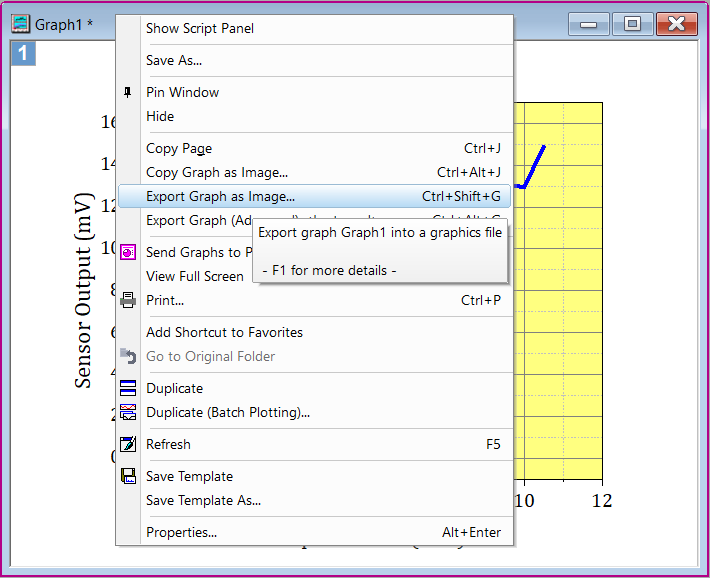
\includegraphics[width=0.45\textwidth]{figures/fig_plot-basic-custom-15.png}
					\hfill
					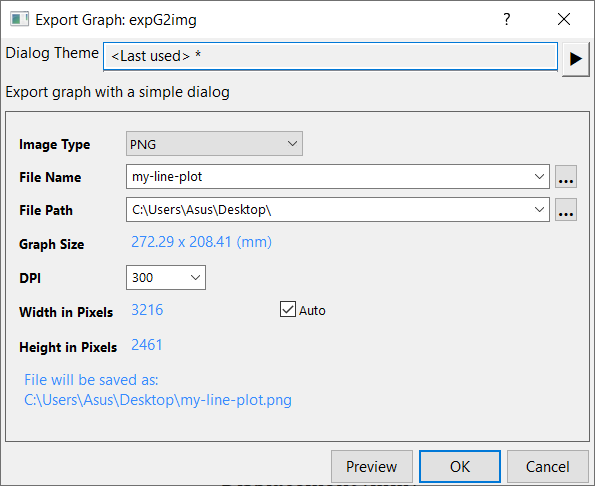
\includegraphics[width=0.45\textwidth]{figures/fig_plot-basic-custom-16.png}
				\end{figure}
				
				\item Finally we obtain the plot file which can now be included in a document as required.
				\begin{figure}[h!]
					\centering
					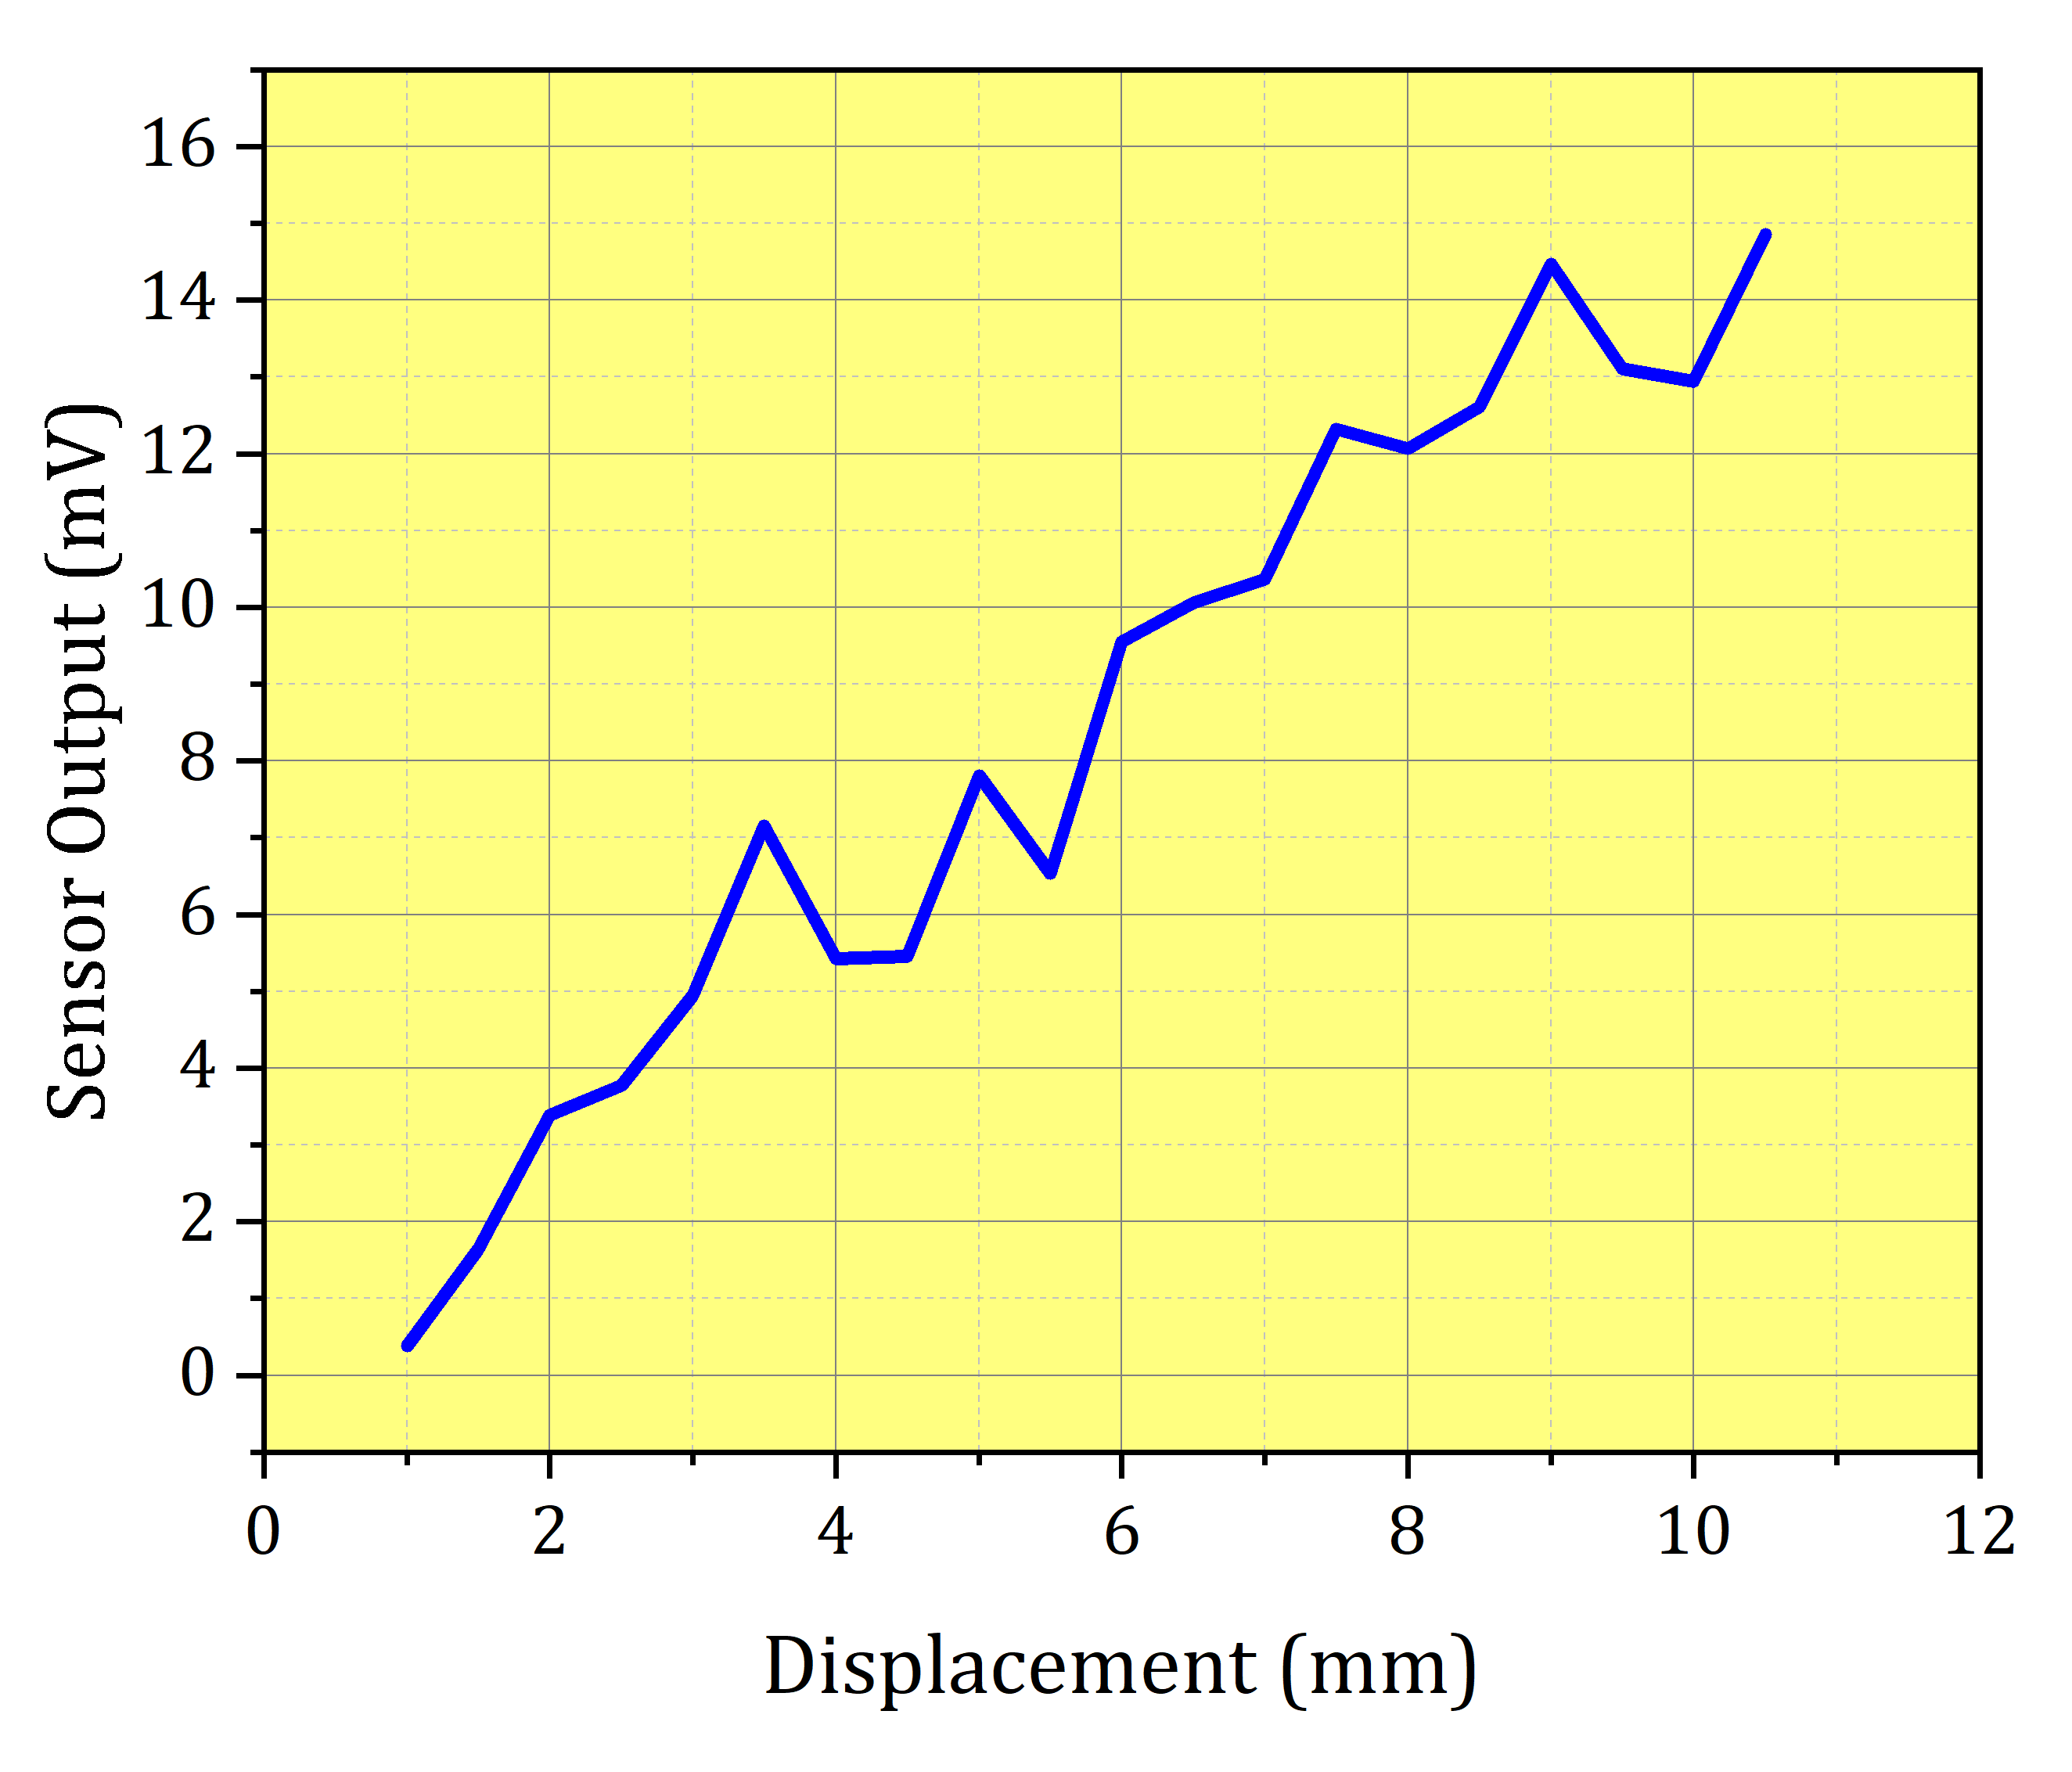
\includegraphics[width=0.6\textwidth,frame]{figures/fig_plot-basic-custom-17.png}
				\end{figure}
			\end{enumerate}
			
	\newpage
	\subsection{Using graph templates}
		A template is a pre-made pattern, model, or mold used as a guide to make multiple identical or similar things. Origin allows us to prepare a graph template based on a graph which is customized according to our requirements. Then later, we can use this template to quickly make identical customizations on other graphs.
		
		\subsubsection{Creating a graph template}
			\begin{enumerate}[I.]
				\item We start with a graph that we have customized as per our requirement.
				\begin{figure}[h!]
					\centering
					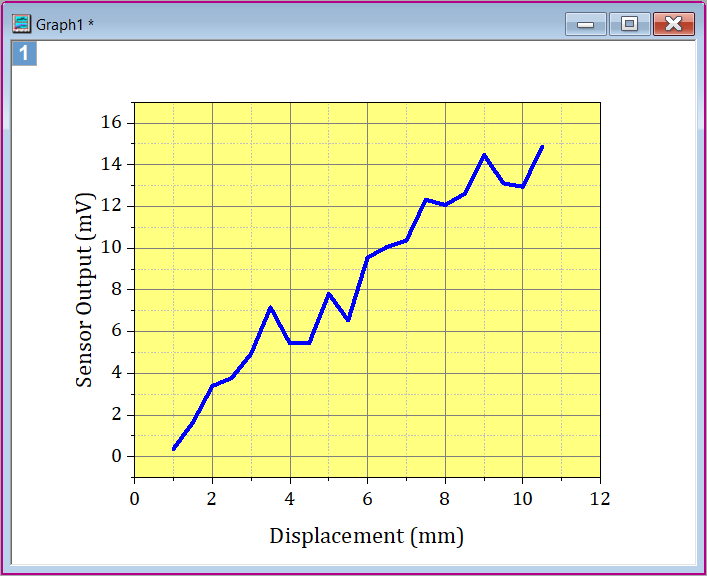
\includegraphics[width=0.6\textwidth]{figures/fig_graph-template-01.png}
				\end{figure}
				
				\item To use this graph as a template, we right-click on the graph's title bar, and then click on \verb|Save Template As...| from the context menu.
				\begin{figure}[h!]
					\centering
					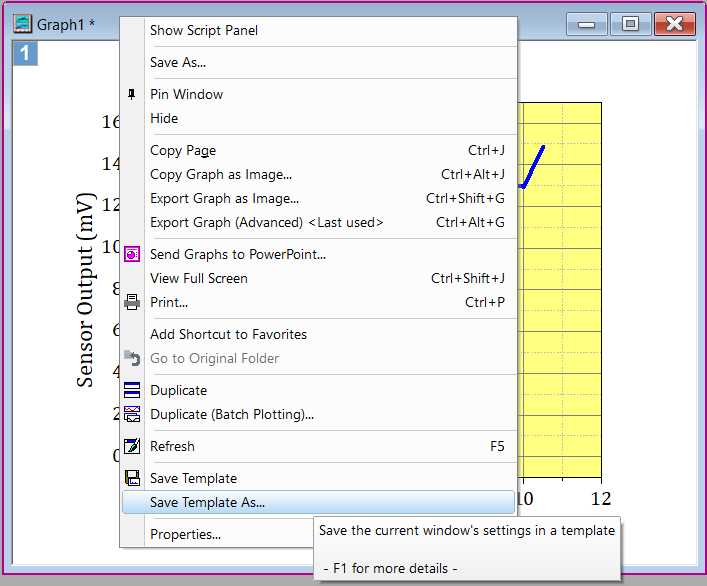
\includegraphics[width=0.5\textwidth]{figures/fig_graph-template-02.png}
				\end{figure}
				
				\newpage
				\item In the save template dialog, we enter the name of the template,\\ for example \verb|Template Name = My Line|. Then we click \verb|OK|.
				\begin{figure}[h!]
					\centering
					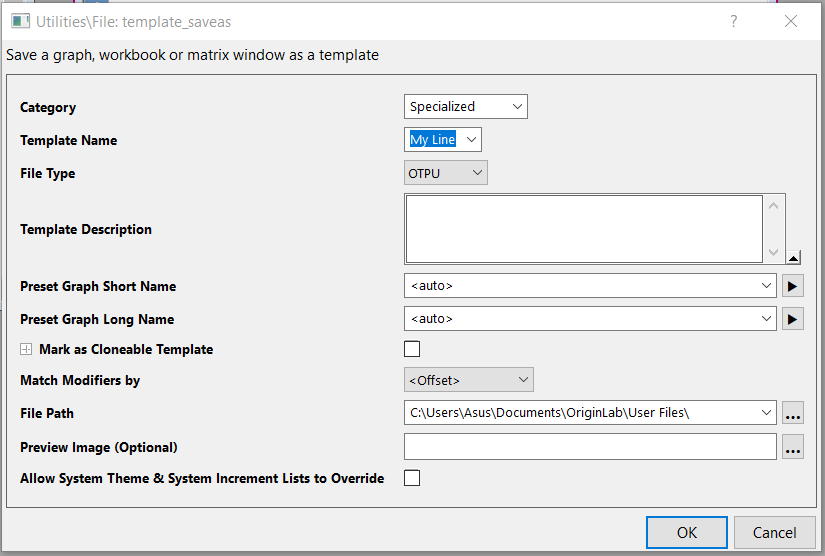
\includegraphics[width=0.5\textwidth]{figures/fig_graph-template-03.png}
				\end{figure}
			\end{enumerate}
			
		\subsubsection{Applying a graph template}
			\begin{enumerate}
				\item Suppose in a different Origin workbook, we wish to plot some other graph using the above template. For example, we can drag and drop the \verb|Exponential Decay.dat| file from the \verb|Samples| \verb|>| \verb|Curve Fitting| folder into the workbook.
				\begin{figure}[h!]
					\centering
					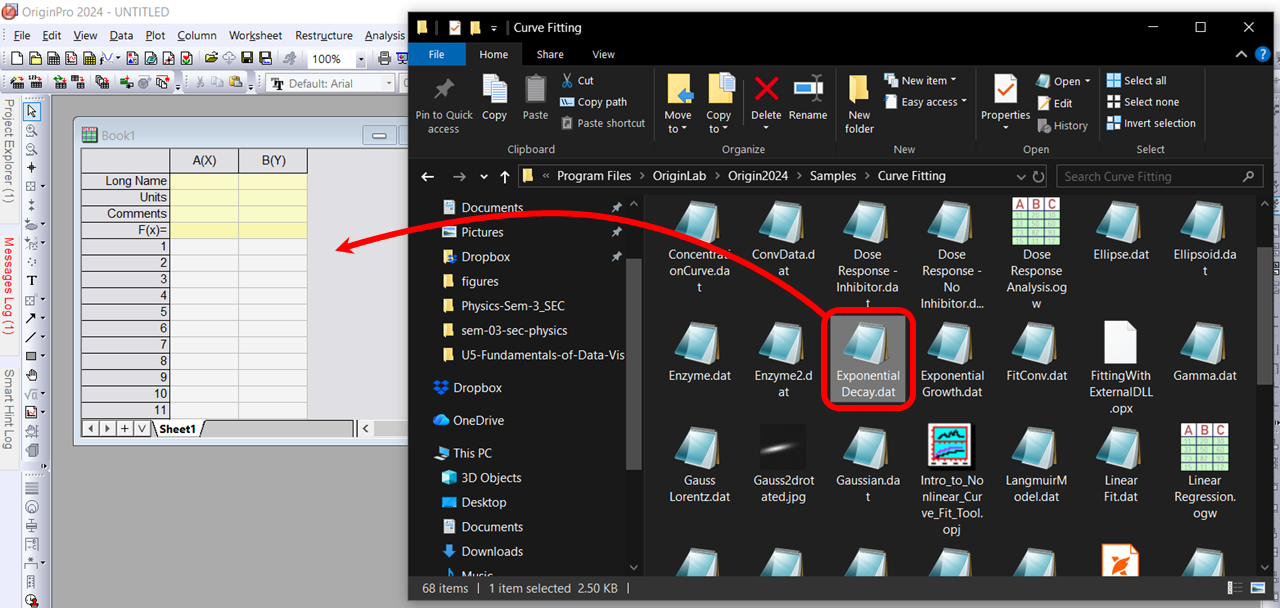
\includegraphics[width=0.8\textwidth]{figures/fig_graph-template-04.png}
				\end{figure}
				
				\newpage
				\item In order to plot the data in column C, we click on that column's header. Then from the main menu, we click \verb|Plot| \verb|>| \verb|User Templates| \verb|>| \verb|My Line|.
				\begin{figure}[h!]
					\centering
					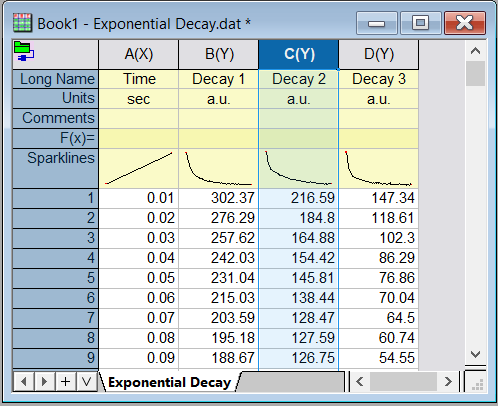
\includegraphics[width=0.4\textwidth]{figures/fig_graph-template-05.png}
					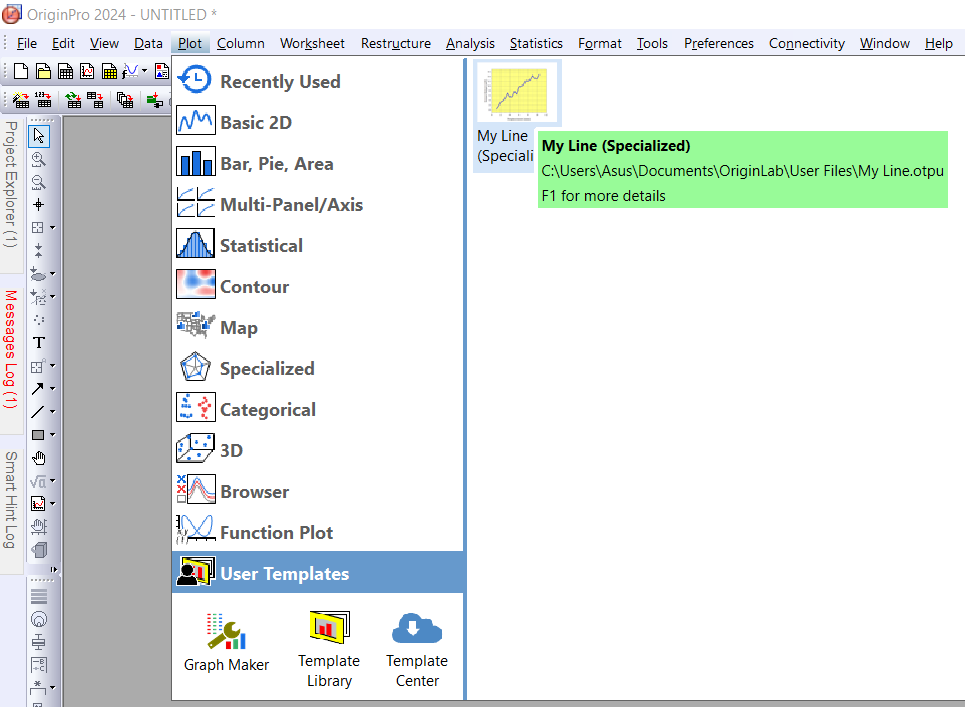
\includegraphics[width=0.5\textwidth]{figures/fig_graph-template-06.png}
				\end{figure}
				
				\item This gives us the desired plot which is customized as per the saved graph template. We can find that the plotting style of this graph is identical to the one which we started with.
				\begin{figure}[h!]
					\centering
					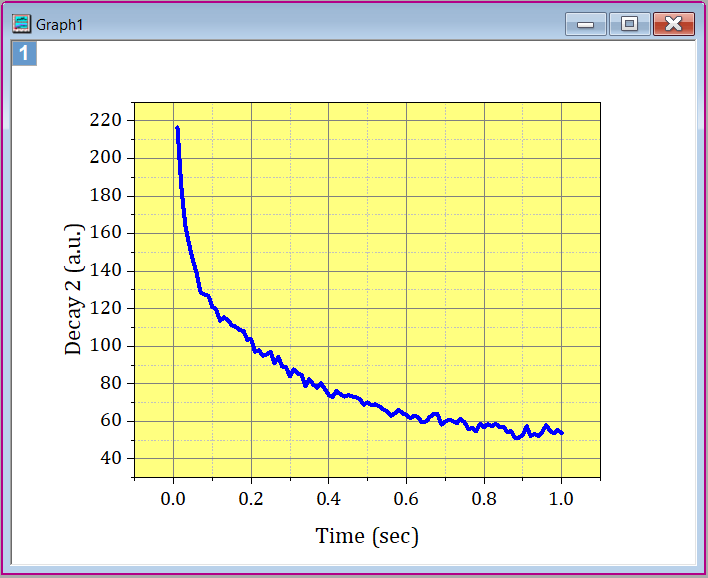
\includegraphics[width=0.6\textwidth]{figures/fig_graph-template-07.png}
				\end{figure}
			\end{enumerate}
	
	%\subsection{Batch plotting}